% \subsection{NGUYÊN HÀM CÓ ĐIỀU KIỆN}
\begin{dang}{Tìm nguyên hàm khi biết giá trị nguyên hàm}
	Phương pháp: Tìm $F(x)=\int f(x)\mathrm{\,d}x$. Sau đó dựa vào $F(x_0)=a$ để suy ra $C$.
\end{dang}
\Opensolutionfile{ans}[ans/ans-C4B1CD2-LC]
% \TN
\begin{ex}%[2D4H2-2]
Hàm số $F(x)$ là một nguyên hàm của hàm số $f(x)=\dfrac{1}{x}$ trên $(-\infty;0)$ thỏa mãn $F(-2)=0$. Khẳng định nào sau đây \textbf{đúng}?
\choice
{\True $F(x)=\ln \left(-\dfrac{x}{2} \right),\,\forall x\in (-\infty;0)$}
{$F(x)=\ln \left|x\right|+C,\,\forall x\in (-\infty;0)$ với $C$ là một số thực bất kì}
{$F(x)=\ln \left|x\right|+\ln 2,\,\forall x\in (-\infty;0)$}
{$F(x)=\ln \left(-x\right)+C,\,\forall x\in (-\infty;0)$ với $C$ là một số thực bất kì}
\loigiai{
Ta có $F(x)=\displaystyle\int \dfrac{1}{x}\mathrm{\,d}x=\ln \left|x\right|+C=\ln (-x)+C,\,\forall x\in (-\infty;0)$.\\
Lại có $F(-2)=0\Rightarrow \ln 2+C=0\Rightarrow C=-\ln 2$.\\
Do đó $F(x)=\ln (-x)-\ln 2=\ln \left(-\dfrac{x}{2}\right)$.
}
\end{ex}

\begin{ex}%[2D4H2-4]
Biết $F(x)$ là một nguyên hàm của hàm số $f(x)=e^{2x}$ và $F(0)=0$. Giá trị của $F(\ln 3)$ bằng
\choice
{$2$}
{$6$}
{$8$}
{\True $4$}
\loigiai{
Ta có $F(x)=\displaystyle\int e^{2x}\mathrm{\,d}x=\dfrac{1}{2}e^{2x}+C$.\\
Lại có $F(0)=0\Rightarrow \dfrac{1}{2}+C=0\Rightarrow C=-\dfrac{1}{2}$.\\
Do đó $F(\ln 3)=\dfrac{1}{2}e^{2\ln 3}-\dfrac{1}{2}=4$.
}
\end{ex}

\begin{ex}%[2D4H2-4]
Cho $F(x)$ là một nguyên hàm của $f(x)=2^x+x+1$. Biết $F(0)=1$. Giá trị của $F(-1)$ bằng
\choice
{$F(-1)=\dfrac{1}{2\ln 2}$}
{\True $F(-1)=\dfrac{1}{2}-\dfrac{1}{2\ln 2}$}
{$F(-1)=1+\dfrac{1}{2\ln 2}$}
{$F(-1)=\dfrac{1}{2}-\dfrac{1}{\ln 2}$}
\loigiai{
Ta có $F(x)=\displaystyle\int (2^x+x+1)\mathrm{\,d}x=\dfrac{2^x}{\ln 2}+\dfrac{x^2}{2}+x+C$.\\
Lại có $F(0)=1\Rightarrow \dfrac{1}{\ln 2}+C=1\Rightarrow C=1-\dfrac{1}{\ln 2}$.\\
Do đó $F(-1)=\dfrac{1}{2\ln 2}+\dfrac{1}{2}-1+1-\dfrac{1}{\ln 2}=\dfrac{1}{2}-\dfrac{1}{2\ln 2}$.
}
\end{ex}

\begin{ex}%[2D4H2-3]
Tìm nguyên hàm $F(x)$ của hàm số $f(x)=\sin x+\cos x$ thoả mãn $F\left(\dfrac{\pi}{2}\right)=2$.
\choice
{$F(x)=-\cos x+\sin x+3$}
{$F(x)=-\cos x+\sin x-1$}
{\True $F(x)=-\cos x+\sin x+1$}
{$F(x)=\cos x-\sin x+3$}
\loigiai{
Ta có $F(x)=\displaystyle\int (\sin x+\cos x)\mathrm{\,d}x=-\cos x+\sin x+C$.\\
Lại có $F\left(\dfrac{\pi}{2}\right)=2\Rightarrow -\cos\dfrac{\pi}{2}+\sin\dfrac{\pi}{2}+C=2\Rightarrow C=1$.\\
Do đó $F(x)=-\cos x+\sin x+1$.
}
\end{ex}

\begin{ex}%[2D4H2-4]
Cho $F(x)$ là một nguyên hàm của hàm số $f(x)=e^x+2x$ thỏa mãn $F(0)=\dfrac{3}{2}$. Tìm $F(x)$.
\choice
{\True $F(x)=e^x+x^2+\dfrac{1}{2}$}
{$F(x)=e^x+x^2+\dfrac{5}{2}$}
{$F(x)=e^x+x^2+\dfrac{3}{2}$}
{$F(x)=e^x+x^2-\dfrac{1}{2}$}
\loigiai{
Ta có $F(x)=\displaystyle\int (e^x+2x)\mathrm{\,d}x=e^x+x^2+C$.\\
Lại có $F(0)=\dfrac{3}{2}\Rightarrow 1+C=\dfrac{3}{2}\Rightarrow C=\dfrac{1}{2}$.\\
Do đó $F(x)=e^x+x^2+\dfrac{1}{2}$.
}
\end{ex}

\begin{ex}%[2D4H2-2]
Cho hàm số $f(x)=\heva{&2x-1&\text{khi}\quad&x\ge 1\\&3x^2-2&\text{khi}\quad&x<1}$, giả sử $F$ là nguyên hàm của  $f$ trên $\mathbb{R}$ thỏa mãn $F(0)=2$. Giá trị của $F(-1)+2F(2)$ bằng
\choice
{\True $9$}
{$15$}
{$11$}
{$6$}
\loigiai{
Ta có $\displaystyle\int (2x-1)\mathrm{\,d}x=x^2-x+C_1$ và $\displaystyle\int (3x^2-2)\mathrm{\,d}x=x^3-2x+C_2$.\\
Suy ra $F(x)=\displaystyle\int f(x)\mathrm{\,d}x=\heva{&x^2-x+C_1&\text{khi}\quad&x\ge 1\\&x^3-2x+C_2&\text{khi}\quad&x<1.}$ 
Lại có $F(0)=2\Rightarrow C_2=2$.\\
Mặt khác hàm số $F$ là nguyên hàm của $f$ trên $\mathbb{R}$ nên $y=F(x)$ liên tục tại $x=1$.\\
Suy ra  $\lim\limits_{ x\to 1^{+}} F(x)=\lim\limits_{ x\to 1^{-}} F(x)\Rightarrow C_1=1$.\\
Khi đó ta có $F(x)=\heva{&x^2-x+1&\text{khi}\quad&x\ge 1\\&x^3-2x+2&\text{khi}\quad&x<1}\Rightarrow \heva{&F(-1)=3\\&F(2)=3.}$  \\
Vậy $F(-1)+2F(2)=9$.  
}
\end{ex}

\Opensolutionfile{ans}[ans/ans-C4B1CD2-CAU7_8-LC]
\setcounter{ex}{6}
\begin{ex}%[2D4H1-2]
	Cho hàm số $f(x)=\heva{&2x+3 &\text{khi } &x\ge 1\\ &3x^2+2 &\text{khi } &x<1.}$ Giả sử $F$ là nguyên hàm của hàm số $f$ trên $\mathbb{R}$ thỏa mãn $F(0)=2$. Giá trị của $F(-1)+2F(2)$ bằng
	\choice
	{$23$}
	{$11$}
	{$10$}	 
	{\True $21$}
	\loigiai{
		Khi $x\ge 1$ thì $F(x)=\displaystyle\int f(x)\mathrm{\,d}x=\displaystyle\int (2x+3)\mathrm{\,d}x=x^2+3x+\mathrm{C}_1$.\\
		Khi $x<1$ thì $F(x)=\displaystyle\int f(x)\mathrm{\,d}x=\displaystyle\int (3x^2+2)\mathrm{\,d}x=x^3+2x+C_2$.\\
		Theo giả thiết $F(0)=2 \Rightarrow C_2=2$.\\
		Ta có $\lim\limits_{x \to 1^+} f(x)=\lim\limits_{x \to 1^-} f(x)=f(1)=5$ nên hàm số $f(x)$ liên tục tại $x=1$.\\
		Suy ra hàm số $f(x)$ liên tục trên $\mathbb{R}$.\\
		Do đó hàm số $F(x)$ liên tục trên $\mathbb{R} \Rightarrow \lim\limits_{x \to 1^+} F(x)=\lim\limits_{x \to 1^-} F(x) \Rightarrow C_1+4=C_2+3 \Rightarrow C_1=1$.\\
		Vậy $F(-1)+2F(2)=-3+C_2+2(10+C_1)=21$.
	}
\end{ex}
\begin{ex}%[2D4H1-2]
	Cho hàm số $f(x)=\heva{&2x+2 &\text{khi } &x\ge 1\\ &3x^2+1 &\text{khi } &x<1.}$ Giả sử $F$ là nguyên hàm của hàm số $f$ trên $\mathbb{R}$ thỏa mãn $F(0)=2$. Giá trị của $F(-1)+2F(2)$ bằng
	\choice
	{\True $18$}
	{$20$}
	{$9$}	 
	{$24$}
	\loigiai{
		$F$ là nguyên hàm của $f$ trên $\mathbb{R}$ nên $F(x)=\heva{&x^2+2x+C_1 &\text{khi } &x\ge 1\\ &x^3+x+C_2 &\text{khi } &x<1.}$\\
		Ta có $F(0)=2 \Rightarrow C_2=2$. \quad $(1)$\\
		Do $F$ liên tục tại $x=1$ nên $\lim\limits_{x \to 1^+} F(x)=\lim\limits_{x \to 1^-} F(x)=F(1)$.\\
		$\Leftrightarrow C_1+3=C_2+2 \mathop  \Leftrightarrow \limits^{(1)} C_1+3=4 \Leftrightarrow C_1=1$.\\
		Do đó $F(x)=\heva{&x^2+2x+1 &\text{khi } &x\ge 1\\ &x^3+x+2 &\text{khi } &x<1.}$\\
		Suy ra $F(-1)+2F(2)=18$.
	}
\end{ex}

\begin{ex}%[2D4H1-2]
	Cho hàm số $y=f(x)$ có đạo hàm là $f'(x)=12x^2+2, \forall x\in \mathbb{R}$ và $f(1)=3$. Biết $F(x)$ là nguyên hàm của $f(x)$ thỏa mãn $F(0)=2$, khi đó $F(1)$ bằng
	\choice
	{$-3$}
	{\True $1$}
	{$2$}
	{$7$}
	\loigiai{
		Ta có $f'(x)=12x^2+2, \forall x\in \mathbb{R} \Rightarrow f(x)=4x^3+2x+C_1$.\\
		Mà $f(1)=3\Rightarrow 3=6+C_1\Rightarrow C_1=-3\Rightarrow f(x)=4x^3+2x-3\Rightarrow F(x)=x^4+x^2-3x+C_2$.\\
		Lại có $F(0)=2\Rightarrow C_2=2\Rightarrow F(x)=x^4+x^2-3x+2$.\\
		Do đó $F(1)=1$.\\
		\textbf{Cách khác:}\\
		Ta có $F(1)=\displaystyle \int\limits_0^1 {f(x)\mathrm{\,d}x}+F(0)=\displaystyle \int\limits_0^1{(4x^3+2x-3)\mathrm{\,d}x}+2=-1+2=1$.}
\end{ex}
\begin{ex}%[2D4H1-3]
	Cho hàm số $f(x)$ thỏa mãn $f'(x)=3-5\sin x$ và $f(0)=10$. Mệnh đề nào dưới đây \textbf{đúng}?
	\choice
	{$f(x)=3x-5\cos x+15$}
	{$f(x)=3x-5\cos x+2$}
	{\True $f(x)=3x+5\cos x+5$}
	{$f(x)=3x+5\cos x+2$}
	\loigiai{
		Ta có $f(x)=\displaystyle \int (3-5\sin x)\mathrm{\,d}x=3x+5\cos x+C$.\\
		Theo giả thiết $f(0)=10$ nên $5+C=10\Rightarrow C=5$.\\
		Vậy $f(x)=3x+5\cos x+5$.
	}
\end{ex}
\begin{ex}%[2D4H1-4]
	Hàm số $f(x)$ có đạo hàm liên tục trên $\mathbb{R}$ và $f'(x)=2\mathrm{e}^{2x}+1, \forall x; f(0)=2$. Hàm $f(x)$ là
	\choice
	{$y=2\mathrm{e}^x+2x$}
	{$y=2\mathrm{e}^x+2$}
	{$y=\mathrm{e}^{2x}+x+2$}
	{\True $y=\mathrm{e}^{2x}+x+1$}
	\loigiai{
		Ta có $\displaystyle \int f'(x)\mathrm{\,d}x=\displaystyle \int(2\mathrm{e}^{2x}+1)\mathrm{\,d}x=\mathrm{e}^{2x}+x+C$.\\
		Suy ra $f(x)=\mathrm{e}^{2x}+x+C$.\\
		Theo bài ra ta có $f(0)=2\Rightarrow 1+C=2\Leftrightarrow C=1$.\\
		Vậy $f(x)=\mathrm{e}^{2x}+x+1$.
	}
\end{ex}
\begin{ex}%[2D4H1-3]
	Cho hàm số $f(x)$ thỏa mãn $f'(x)=2-5\sin x$ và $ f(0)=10$. Mệnh đề nào dưới đây \textbf{đúng}?
	\choice
	{$f(x)=2x+5\cos x+3$}
	{$f(x)=2x-5\cos x+15$}
	{\True $f(x)=2x+5\cos x+5$}
	{$f(x)=2x-5\cos x+10$}
	\loigiai{
		Ta có $f(x)=\displaystyle \int f'(x)\mathrm{\,d}x=\displaystyle\int (2-5\sin x)\mathrm{\,d}x=2x+5\cos x+C$.\\
		Mà $f(0)=10$ nên $5+C=10\Rightarrow C=5$.\\
		Vậy $f(x)=2x+5\cos x+5$.}
\end{ex}
\begin{ex}%[2D4V1-2]
	Cho hàm số $f(x)$ thỏa mãn $f'(x)=ax^2+\dfrac{b}{x^3}$, $f'(1)=3$, $f(1)=2$, $f\left(\dfrac{1}{2}\right)=-\dfrac{1}{12}$. Khi đó $2a+b$ bằng
	\choice
	{$-\dfrac{3}{2}$}
	{$0$}
	{\True $5$}
	{$\dfrac{3}{2}$}
	\loigiai{
		Ta có $f'(1)=3\Rightarrow a+b=3. \quad (1)$\\
		Hàm số có đạo hàm liên tục trên khoảng $(0;+\infty)$, các điểm $x=1$, $x=\dfrac{1}{2}$ đều thuộc $(0;+\infty)$ nên\\
		$f(x)=\displaystyle \int f'(x)\mathrm{\,d}x=\displaystyle \int (ax^2+\dfrac{b}{x^3})\mathrm{\,d}x=\dfrac{ax^3}{3}-\dfrac{b}{2x^2}+C$.\\
		\begin{itemize}
			\item $f(1)=2\Rightarrow \dfrac{a}{3}-\dfrac{b}{2}+C=2. \quad (2)$
			\item $f\left(\dfrac{1}{2}\right)=-\dfrac{1}{12}\Rightarrow \dfrac{a}{24}-2b+C=-\dfrac{1}{12}. \quad (3)$
		\end{itemize}
		Từ $(1)$, $(2)$ và $(3)$ ta được hệ phương trình $\heva{ &a+b=3\\ &\dfrac{a}{3}-\dfrac{b}{2}+C=2\\ &\dfrac{a}{24}-2b+C=-\dfrac{1}{12}}\Leftrightarrow \heva{&a=2\\ &b=1\\ &C=\dfrac{11}{6}.}$\\
		Vậy $2a+b=2\cdot 2+1=5$.
	}
\end{ex}
\begin{ex}%[2D4V1-2]
	Tìm một nguyên hàm $F(x)$ của hàm số $f(x)=ax+\dfrac{b}{x^2} \quad (x\ne  0)$, biết rằng $F(-1)=1$, $F(1)=4$, $f(1)=0$.
	\choice
	{$F(x)=\dfrac{3}{2}x^2+\dfrac{3}{4x}-\dfrac{7}{4}$}
	{$F(x)=\dfrac{3}{4}x^2-\dfrac{3}{2x}-\dfrac{7}{4}$}
	{\True $F(x)=\dfrac{3}{4}x^2+\dfrac{3}{2x}+\dfrac{7}{4}$}
	{$F(x)=\dfrac{3}{2}x^2-\dfrac{3}{2x}-\dfrac{1}{2}$}
	\loigiai{
		Ta có $F(x)=\displaystyle \int f(x)\mathrm{\,d}x=\displaystyle \int \left(ax+\dfrac{b}{x^2}\right)\mathrm{\,d}x=\dfrac{1}{2}ax^2-\dfrac{b}{x}+C$.\\
		Theo bài ra $\heva{&F(-1)=1\\ &F(1)=4\\ &f(1)=0}\Leftrightarrow \heva{&\dfrac{1}{2}a+b+C=1\\ &\dfrac{1}{2}a-b+C=4\\ &a+b=0} \Leftrightarrow \heva{&b=-\dfrac{3}{2}\\ &a=\dfrac{3}{2}\\ &C=\dfrac{7}{4}.} $\\
		Vậy $F(x)=\dfrac{3}{4}{x^2}+\dfrac{3}{2x}+\dfrac{7}{4}$.
	}
\end{ex}
\begin{ex}%[2D4V1-2]
	Cho hàm số $f(x)$ xác định trên $\mathbb{R}\setminus \{0\}$ thỏa mãn $f'(x)=\dfrac{x+1}{x^2}$, $f(-2)=\dfrac{3}{2}$ và $f(2)=2\ln 2-\dfrac{3}{2}$. Giá trị của biểu thức $f(-1)+f(4)$ bằng
	\choice
	{$\dfrac{6\ln 2-3}{4}$}
	{$\dfrac{6\ln 2+3}{4}$}
	{\True $\dfrac{8\ln 2+3}{4}$}
	{$\dfrac{8\ln 2-3}{4}$}
	\loigiai{
		Có $f(x)=\displaystyle \int f'(x)\mathrm{\,d}x=\displaystyle \int \dfrac{x+1}{x^2}\mathrm{\,d}x=\ln x-\dfrac{1}{x}+C$.\\
		Tìm được $f(x)=\heva{&\ln |x|-\dfrac{1}{x}+C_1 &\text{khi } &x<0\\ &\ln |x|-\dfrac{1}{x}+C_2 &\text{khi } &x>0.}$\\
		Do $f(-2)=\dfrac{3}{2} \Rightarrow \ln 2+\dfrac{1}{2}+C_1=\dfrac{3}{2} \Rightarrow C_1=1-\ln 2$.\\
		Do $f(2)=2\ln 2-\dfrac{3}{2} \Rightarrow \ln 2-\dfrac{1}{2}+C_2=2\ln 2-\dfrac{3}{2} \Rightarrow C_2=\ln 2-1$.\\
		Suy ra $f(x)=\heva{&\ln |x|-\dfrac{1}{x}+1-\ln 2 &\text{khi } &x<0\\ &\ln |x|-\dfrac{1}{x}+\ln 2-1 &\text{khi } &x>0.}$\\
		Vậy $f(-1)+f(4)=(2-\ln 2)+\left(\ln 4-\dfrac{1}{4}+\ln 2-1\right)=\dfrac{8\ln 2+3}{4}$.
	}
\end{ex}

\begin{ex}%[2D4V1-2]
	\immini{Cho hàm số $y=f(x)$. Đồ thị của hàm số \break $y=f'(x)$ trên $[-5 ; 3]$ như hình vẽ (phần cong của đồ thị là một phần của parabol \break $y=a x^2+b x+c$). Biết $f(0)=0$, giá trị của $2 f(-5)+3 f(2)$ bằng
		\choice
		{$33$}
		{$\dfrac{109}{3}$}
		{\True $\dfrac{35}{3}$}
		{$11$}
	}{
		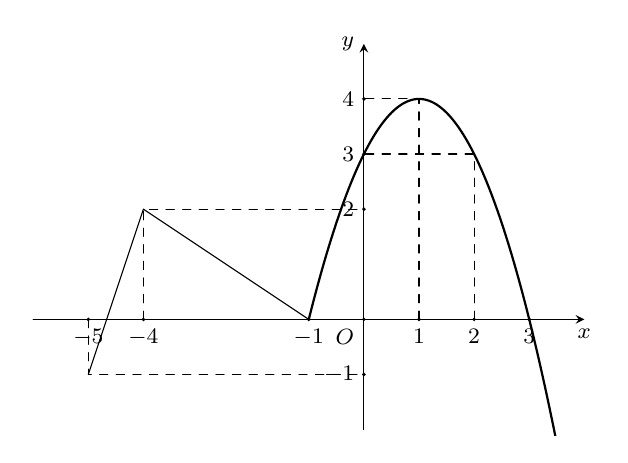
\begin{tikzpicture}[scale=0.7, font=\footnotesize, line join=round, line cap=round,>=stealth]
			%Gán số liệu.
			\def\xmin{-6};\def\ymin{-2};\def\xmax{4};\def\ymax{5};
			%Gán tọa độ.
			\coordinate (O) at (0,0);
			%Trục Oxy.
			\draw[->] (\xmin,0)--(\xmax,0) node[below]{$x$};
			\draw[->] (0,\ymin)--(0,\ymax) node[left]{$y$};
			\fill (O) node[below left]{$O$} circle(1pt);
			%Giới hạn đồ thị.
			\clip ({\xmin-0.1},{\ymin-0.1}) rectangle ({\xmax+0.1},{\ymax+0.1});
			\foreach \x in {-5,-4,-1,1,2,3}{
					\fill (\x,0) node[below]{$\x$} circle(1pt);
				}
			\foreach \y in {-1,2,3,4}{
					\fill (0,\y) node[left]{$\y$} circle(1pt);
				}
			\draw (-5,-1)--(-4,2)--(-1,0);
			\draw[thick,samples=100] plot[domain=-1:3.5](\x,{-(\x)^2+2*\x+3});
			\draw[dashed] (-5,0)|-(0,-1) (-4,0)|-(0,2) (1,0)|-(0,4) (2,0)|-(0,3);
		\end{tikzpicture}
	}
	\loigiai{
		Parabol $y=a x^2+b x+c$ qua các điểm $(2 ; 3)$, $(1 ; 4)$, $(0 ; 3)$, $(-1 ; 0)$, $(3 ; 0)$ nên xác định được $y=-x^2+2 x+3$, $\forall x \geq-1$ suy ra $f(x)=-\dfrac{x^3}{3}+x^2+3 x+C_1$.\\
		Mà $f(0)=0 \Rightarrow C_1=0$, $f(x)=-\dfrac{x^3}{3}+x^2+3 x$.\\
		Có $f(-1)=-\dfrac{5}{3}$, $ f(2)=\dfrac{22}{3}$.\quad $(1)$\\
		Đồ thị $f'(x)$ trên đoạn $[-4 ;-1]$ qua các điểm $(-4 ; 2)$, $(-1 ; 0)$.\\
		Nên $f'(x)=-\dfrac{2}{3}(x+1) \Rightarrow f(x)=-\dfrac{2}{3}\left(\dfrac{x^2}{2}+x\right)+C_2$.\\
		Mà $f(-1)=-\dfrac{5}{3} \Leftrightarrow C_2=-\dfrac{5}{3}+\dfrac{2}{3}\left(-\dfrac{1}{2}\right)=-2 \Rightarrow f(x)=-\dfrac{2}{3}\left(\dfrac{x^2}{2}+x\right)-2$, hay $f(-4)=-\dfrac{14}{3}$.\\
		Đồ thị $f'(x)$ trên đoạn $[-5 ;-4]$ qua các điểm $(-4 ; 2)$, $(-5 ;-1)$.\\
		Nên $f'(x)=3 x+14 \Rightarrow f(x)=\dfrac{3 x^2}{2}+14 x+C_3$.\\
		Mà $f(-4)=-\dfrac{14}{3} \Leftrightarrow \dfrac{3 \cdot(-4)^2}{2}+14 \cdot(-4)+C_3=-\dfrac{14}{3}$ suy ra $C_3=\dfrac{82}{3}$.\\
		Ta có $f(x)=\dfrac{3 x^2}{2}+14 x+\dfrac{82}{3} \Rightarrow f(-5)=-\dfrac{31}{6}$.\quad $(2)$\\
		Từ $(1)$ và $(2)$ ta được $2 f(-5)+3 f(2)=-\dfrac{31}{3}+22=\dfrac{35}{3}$.
	}
\end{ex}
\begin{ex}%[2D4H1-4]
	Cho hàm số $f(x)=2x+\mathrm{e}^x$. Một nguyên hàm $F(x)$ của hàm số $f(x)$ thỏa mãn $F(0)=2024$. Biết $F(x)=ax^2+b\mathrm{e}^x+c$, giá trị của $a+b+c$ là
	\shortans{$2025$}
	\loigiai{
		Ta có $\displaystyle\int f(x)\mathrm{\,d}x=\displaystyle\int (2x+\mathrm{e}^x)\mathrm{\,d}x=x^2+\mathrm{e}^x+C$.\\
		Có $F(x)$ là một nguyên hàm của $f(x)$ và $F(0)=2024$.\\
		Tìm được $\heva{&F(x)=x^2+\mathrm{e}^x+C\\ &F(0)=2024} \Rightarrow 1+C=2024 \Leftrightarrow C=2023$.\\
		Suy ra $F(x)=x^2+\mathrm{e}^x+2023$.\\
		Vậy $a+b+c=2025$.
	}
\end{ex}
% \begin{ex}%[2D4H1-3]
% 	Cho $F(x)$ là một nguyên hàm của hàm số $f(x)=\sin x+1$ biết $F\left( \dfrac{\pi}{6}\right) =0$. Tính giá trị của $F(\pi)$. (Làm tròn đến chữ số thập phân thứ hai)
% 	\shortans{$4{,}48$}
% 	\loigiai{
% 		$F(x)=\displaystyle \int(\sin x+1)\mathrm{\,d}x=x-\cos x+C$.\\
% 		Do $F\left( \dfrac{\pi}{6}\right) =0 \Rightarrow \dfrac{\pi}{6}-\cos \left( \dfrac{\pi}{6}\right) +C=0\Leftrightarrow C=\dfrac{\sqrt{3}}{2}-\dfrac{\pi}{6}$.\\
% 		Suy ra $F(x)=x-\cos x+\dfrac{\sqrt{3}}{2}-\dfrac{\pi}{6}$.\\
% 		Vậy $F(\pi)=4{,}48$. 
% 	}
% \end{ex}
% \begin{ex}%[2D4H1-2]
% 	Cho $F(x)$ là một nguyên hàm của $f(x)=(5x+3)^5$. Biết $F(1)=0$. Tính giá trị của $\sqrt{|F(0)|}$. (Làm tròn đến chữ số thập phân thứ nhất)
% 	\shortans{$93{,}3$}
% 	\loigiai{
% 		Ta có $F(x)=\displaystyle \int f(x)\mathrm{\,d}x=\displaystyle \int (5x+3)^5\mathrm{\,d}x=\dfrac{(5x+3)^6}{30}+C$.\\
% 		Do $F(1)=0\Rightarrow 0=\dfrac{(5\cdot 1+3)^6}{30}+C\Rightarrow C=-\dfrac{131072}{15}$.\\
% 		Suy ra $F(x)=\dfrac{(5x+3)^6}{30}-\dfrac{131072}{15}$.\\
% 		Do đó $F(0)=\dfrac{(5\cdot 0+3)^6}{30}-\dfrac{131072}{15}=-\dfrac{52283}{6}$.\\
% 		Vậy $\sqrt{|F(0)|}=93{,}3$.
% 	}
% \end{ex}
% \begin{ex}%[2D4H1-2]
% 	Cho $F(x)$ là một nguyên hàm của $f(x)=x^3-4x+5$. Biết $F(1)=3$. Tính $|F(0)|$.
% 	\shortans{$0{,}25$}
% 	\loigiai{
% 		Ta có $F(x)=\displaystyle \int f(x)\mathrm{\,d}x=\displaystyle \int(x^3-4x+5)\mathrm{\,d}x=\dfrac{x^4}{4}-2x^2+5x+C$.\\
% 		Do $F(1)=3\Rightarrow 3=\dfrac{1^4}{4}-2\cdot 1^2+5\cdot 1+C\Rightarrow C=-\dfrac{1}{4}$.\\
% 		Suy ra $F(x)=\dfrac{x^4}{4}-2x^2+5x-\dfrac{1}{4}$.\\
% 		Vậy $|F(0)|=0{,}25$.
% 	}
% \end{ex}
% \begin{ex}%[2D4H1-3]
% 	Cho $F(x)$ là một nguyên hàm của $f(x)=3-5\cos x$. Biết $F(\pi )=2$. Tính $F\left(\dfrac{\pi}{2}\right)$. (Làm tròn đến chữ số thập phân thứ nhất)
% 	\shortans{$-7{,}7$}
% 	\loigiai{
% 		Ta có $F(x)=\displaystyle \int f(x)\mathrm{\,d}x=\displaystyle \int(3-5\cos x)\mathrm{\,d}x=3x-5\sin x+C$.\\
% 		Do $F(\pi )=2\Rightarrow 2=3\pi -5\sin \pi+C\Rightarrow C=-3\pi +2$.\\
% 		Suy ra $F(x)=3x-5\sin x-3\pi +2$.\\
% 		Vậy $F\left(\dfrac{\pi}{2}\right)=-7{,}7$.
% 	}
% \end{ex}
% \begin{ex}%[2D4H1-2]
% 	Cho $F(x)$ là một nguyên hàm của $f(x)=\dfrac{3-5x^2}{x}$. Biết $F(\mathrm{e})=1$. Tính $F(2)$. (Làm tròn đến chữ số thập phân thứ hai)
% 	\shortans{$8{,}55$}
% 	\loigiai{
% 		Hàm số $f(x)=\dfrac{3-5x^2}{x}=\dfrac{3}{x}-5x$.\\
% 		Có $F(x)=\displaystyle \int f(x)\mathrm{\,d}x=\displaystyle \int\left(\dfrac{3}{x}-5x\right)\mathrm{\,d}x=3\ln |x|-\dfrac{5}{2} x^2 +C$.\\
% 		Do $F(\mathrm{e})=1\Rightarrow 1=3\ln |\mathrm{e}|-\dfrac{5}{2} \mathrm{e}^2 +C \Rightarrow C=\dfrac{5}{2} \mathrm{e}^2 -2$.\\
% 		Suy ra $F(x)=3\ln |x|-\dfrac{5}{2} x^2 +\dfrac{5}{2} \mathrm{e}^2 -2$.\\
% 		Vậy $F(2)=8{,}55$.
% 	}
% \end{ex}
% \begin{ex}%[2D4H1-2]
% 	Cho $F(x)$ là một nguyên hàm của $f(x)=\dfrac{x^2+1}{x}$. Biết $F(1)=\dfrac{3}{2}$. Tính $F(-1)$.
% 	\shortans{$1{,}5$}
% 	\loigiai{
% 		Hàm số $f(x)=\dfrac{x^2+1}{x}=x+\dfrac{1}{x}$.\\
% 		Có $F(x)=\displaystyle \int f(x)\mathrm{\,d}x=\displaystyle \int\left(x+\dfrac{1}{x}\right)\mathrm{\,d}x=\dfrac{x^2}{2}+\ln |x|+C$.\\
% 		Do $F(1)=\dfrac{3}{2}\Rightarrow \dfrac{3}{2}=\dfrac{1^2}{2}+\ln |1|+C \Rightarrow C=1$.\\
% 		Suy ra $F(x)=\dfrac{x^2}{2}+\ln |x|+1$.\\
% 		Vậy $F(-1)=\dfrac{(-1)^2}{2}+\ln |-1|+1=\dfrac{3}{2}=1{,}5$.
% 	}
% \end{ex}
% \begin{ex}%[2D4H1-2]
% 	Cho $F(x)$ là một nguyên hàm của hàm số $f(x)=\dfrac{x^3-1}{x^2}$. Biết $F(-2)=0$. Tính giá trị của $F(2)$.
% 	\shortans{$1$}
% 	\loigiai{
% 		Hàm số $f(x)=\dfrac{x^3-1}{x^2}=x-\dfrac{1}{x^2}$.\\
% 		Có $F(x)=\displaystyle \int f(x)\mathrm{\,d}x=\displaystyle \int\left(x-\dfrac{1}{x^2}\right)\mathrm{\,d}x=\dfrac{x^2}{2}+\dfrac{1}{x}+C$.\\
% 		Do $F(-2)=0\Rightarrow 0=\dfrac{(-2)^2}{2}+\dfrac{1}{(-2)}+C\Rightarrow C=-\dfrac{3}{2}$.\\
% 		Suy ra $F(x)=\dfrac{x^2}{2}+\dfrac{1}{x}-\dfrac{3}{2}$.\\
% 		Vậy $F(2)=1$.
% 	}
% \end{ex}
% \begin{ex}%[2D4H1-4]
% 	Cho $F(x)$ là một nguyên hàm của hàm số $f(x)=x\sqrt{x}+\dfrac{1}{\sqrt{x}}$. Biết $F(1)=-2$. Tính $F(0)$.
% 	\shortans{$-4{,}4$}
% 	\loigiai{
% 		Hàm số $f(x)=x\sqrt{x}+\dfrac{1}{\sqrt{x}}=x^{\tfrac{3}{2}}+x^{-\tfrac{1}{2}}$.\\
% 		Có $F(x)=\displaystyle \int f(x)\mathrm{\,d}x=\displaystyle \int\left(x^{\tfrac{3}{2}}+x^{-\tfrac{1}{2}}\right)\mathrm{\,d}x=\dfrac{2}{5}x^{\tfrac{5}{2}}+2\sqrt{x}+C$.\\
% 		Do $F(1)=-2\Rightarrow -2=\dfrac{2}{5}\cdot 1^{\tfrac{5}{2}}+2\sqrt{1} +C \Rightarrow C=-\dfrac{22}{5}$.\\
% 		Suy ra $F(x)=\dfrac{2}{5}x^{\tfrac{5}{2}}+2\sqrt{x} -\dfrac{22}{5}$.\\
% 		Vậy $F(0)=-4{,}4$.
% 	}
% \end{ex}
% \begin{ex}%[2D4H1-3]
% 	Cho $F(x)$ là một nguyên hàm của hàm số $f(x)=\sin x +1$. Biết $F\left(\dfrac{\pi}{6}\right)=0$. Tính $F(-1)$. (Làm tròn đến chữ số thập phân thứ nhất)
% 	\shortans{$-1{,}2$}
% 	\loigiai{
% 		Ta có $F(x)=\displaystyle \int f(x)\mathrm{\,d}x=\displaystyle \int(\sin x +1)\mathrm{\,d}x=-\cos x +x +C$.\\
% 		Do $F\left(\dfrac{\pi}{6}\right)=0\Rightarrow 0=-\cos \dfrac{\pi}{6} +\dfrac{\pi}{6} +C\Rightarrow C=-\dfrac{\pi}{6} +\dfrac{\sqrt{3}}{2}$.\\
% 		Suy ra $F(x)=-\cos x +x -\dfrac{\pi}{6} +\dfrac{\sqrt{3}}{2}$.\\
% 		Vậy $F(-1)=-1{,}2$.
% 	}
% \end{ex}
% \begin{ex}%[2D4V1-3]
% 	Cho $F(x)$ là một nguyên hàm của $f(x)=2024-\sin^2 \dfrac{x}{2}$. Biết $F\left(\dfrac{\pi}{2}\right)=2025$. Tính $\sqrt{|F(0)|}$. (Làm tròn đến chữ số thập phân thứ nhất)
% 	\shortans{$34$}
% 	\loigiai{
% 		Hàm số $f(x)=2024-\sin^2 \dfrac{x}{2}=2024-\dfrac{1-\cos x}{2}=\dfrac{4047+\cos x}{2}$.\\
% 		Có $F(x)=\displaystyle \int f(x)\mathrm{\,d}x=\displaystyle \int\left(\dfrac{4047+\cos x}{2}\right)\mathrm{\,d}x=\dfrac{1}{2}(4047x+\sin x)+C$.\\
% 		Do $F\left(\dfrac{\pi}{2}\right)=2025\Rightarrow 2025=\dfrac{1}{2}(4047\cdot \dfrac{\pi}{2} +\sin \dfrac{\pi}{2})+C\Rightarrow C=-\dfrac{4047}{4}\pi +\dfrac{4049}{2}$.\\
% 		Suy ra $F(x)=\dfrac{1}{2}(4047x+\sin x)-\dfrac{4047}{4}\pi +\dfrac{4049}{2}$.\\
% 		Vậy $\sqrt{|F(0)|}=34$.
% 	}
% \end{ex}
% \begin{ex}%[2D4V1-3]
% 	Cho $F(x)$ là một nguyên hàm của $f(x)=\sin^2 \dfrac{x}{4} \cdot \cos^2 \dfrac{x}{4}$. Biết $F\left(\dfrac{\pi}{3}\right)=0$. Tính giá trị của $F(\pi)$. (Làm tròn đến chữ số thập phân thứ hai)
% 	\shortans{$0{,}37$}
% 	\loigiai{
% 		Hàm số $f(x)=\sin^2 \dfrac{x}{4} \cdot \cos^2 \dfrac{x}{4}=\dfrac{1}{8}(1-\cos x)$.\\
% 		Có $F(x)=\displaystyle \int f(x)\mathrm{\,d}x=\displaystyle \int \dfrac{1}{8}(1-\cos x)\mathrm{\,d}x=\dfrac{1}{8}(x-\sin x)+C$.\\
% 		Do $F\left(\dfrac{\pi}{3}\right)=0\Rightarrow 0=\dfrac{1}{8}\left(\dfrac{\pi}{3}-\sin \dfrac{\pi}{3}\right)+C\Rightarrow C=-\dfrac{\pi}{24}+\dfrac{\sqrt{3}}{16}$.\\
% 		Suy ra $F(x)=\dfrac{1}{8}(x-\sin x)-\dfrac{\pi}{24}+\dfrac{\sqrt{3}}{16}$.\\
% 		Vậy $F(\pi)=0{,}37$.
% 	}
% \end{ex}
% \begin{ex}%[2D4H1-2]
% 	Cho hàm số $f(x)=\heva{&2x+5 &\text{khi } &x\ge 1\\ &3x^2+4 &\text{khi } &x<1.}$ Giả sử $F$ là nguyên hàm của $f$ trên $\mathbb{R}$ thỏa mãn $F(0)=2$. Giá trị của $F(-1)+2F(2)$.
% 	\shortans{$27$}
% 	\loigiai{
% 		Ta có $f(x)=\heva{&2x+5 &\text{khi } &x\ge 1\\ &3x^2+4 &\text{khi } &x<1}\Rightarrow \heva{&F(x)=x^2+5x+C_1 &\text{khi } &x\ge 1\\ &F(x)=x^3+4x+C_2 &\text{khi } &x<1.}$\\
% 		Vì $F$ là nguyên hàm của $f$ trên $\mathbb{R}$ thỏa mãn $F(0)=2$ nên $C_2=2\Rightarrow F(x)=x^3+4x+2$.\\
% 		Vì $F(x)$ liên tục trên $\mathbb{R}$ nên $F(x)$ liên tục tại $x=1$ nên:\\
% 		$\lim\limits_{x\to1^+} F(x)=\lim\limits_{x\to1^-} F(x)=F(1)\Rightarrow 6+C_1=7\Rightarrow C_1=1$.\\
% 		Vậy ta có $\heva{&F(x)=x^2+5x+1 &\text{khi } &x\ge 1\\ &F(x)=x^3+4x+2 &\text{khi } &x<1}\Rightarrow F(-1)+2F(2)=27$.
% 	}
% \end{ex}
\begin{ex}%[2D4V1-4]
	Gọi $F(x)$ là một nguyên hàm của hàm số $f(x)=2^x$, thỏa mãn $F(0)=\dfrac{1}{\ln 2}$. Giá trị biểu thức $T=F(0)+F(1)+\cdots +F(2018)+F(2019)$ có dạng $\dfrac{{2^{2020}}+a}{\ln b}$. Giá trị của $\dfrac{a}{b}$ là
	\shortans{$-0{,}5$}
	\loigiai{
		Ta có $\displaystyle \int f(x) \mathrm{\,d}x=\displaystyle \int 2^x \mathrm{\,d}x=\dfrac{2^x}{\ln 2}+C$.\\
		$F(x)$ là một nguyên hàm của hàm số $f(x)=2^x$, ta có $F(x)=\dfrac{2^x}{\ln 2}+C$ mà $F(0)=\dfrac{1}{\ln 2}$.\\
		$\Rightarrow C=0\Rightarrow F(x)=\dfrac{2^x}{\ln 2}$.\\
		\begin{eqnarray*}
			T&=&F(0)+F(1)+\cdots +F(2018)+F(2019)\\
			&=&\dfrac{1}{\ln 2}(1+2+2^2+\cdots +2^{2018}+2^{2019})\\
			&=&\dfrac{1}{\ln 2}\cdot \dfrac{{2^{2020}}-1}{2-1}\\
			&=&\dfrac{{2^{2020}}-1}{\ln 2}.\\
		\end{eqnarray*}
		Vậy $\dfrac{a}{b}=-\dfrac{1}{2}=-0{,}5$
	}
\end{ex}
\begin{ex}%[2D4V1-3]
	Cho $F(x)$ là một nguyên hàm của hàm số $f(x)=\dfrac{1}{\cos^2 x}$. Biết $F\left(\dfrac{\pi}{4}+k\pi \right)=k$ với mọi $k\in \mathbb{Z}$. Tính giá trị của biểu thức $T=F(0)+F(\pi )+F(2\pi )+\cdots +F(10\pi )$.
	\shortans{$44$}
	\loigiai{
		Ta có $\displaystyle \int f(x) \mathrm{\,d}x=\displaystyle \int \dfrac{\mathrm{\,d}x}{\cos^2 x}=\tan x+C$.\\
		Suy ra 
		$F(x)=\heva{&\tan x+C_0, \quad x\in \left(-\dfrac{\pi}{2};\dfrac{\pi}{2}\right)\\ &\tan x+C_1, \quad x\in \left(\dfrac{\pi}{2};\dfrac{3\pi}{2}\right)\\ &\tan x+C_2, \quad x\in \left(\dfrac{3\pi}{2};\dfrac{5\pi}{2}\right)\\ &\cdots\\ &\tan x+C_9, \quad x\in \left(\dfrac{17\pi}{2};\dfrac{19\pi}{2}\right)\\ &\tan x+C_{10}, \quad x\in \left(\dfrac{19\pi}{2};\dfrac{21\pi}{2}\right)}\Rightarrow \heva{&F\left(\dfrac{\pi}{4}+0\pi\right)=1+C_0=0\Rightarrow C_0=-1\\ &F\left(\dfrac{\pi}{4}+\pi\right)=1+C_1=1\Rightarrow C_1=0\\ &F\left(\dfrac{\pi}{4}+2\pi\right)=1+C_2=2\Rightarrow C_2=1\\ &\cdots \\ &F\left(\dfrac{\pi}{4}+9\pi\right)=1+C_9=9\Rightarrow C_9=8\\ &F\left(\dfrac{\pi}{4}+10\pi\right)=1+C_{10}=0\Rightarrow C_{10}=9.}$\\
		Vậy \begin{eqnarray*}
			T&=&F(0)+F(\pi )+F(2\pi )+\cdots +F(10\pi )\\ &=&\tan 0-1+\tan \pi +\tan 2\pi +1+\cdots +\tan 10\pi +9\\ &=&44.
		\end{eqnarray*}
	}
\end{ex}
% \begin{ex}%[2D4V1-3]
% 	Hàm số $f(x)$ có đạo hàm liên tục trên $\mathbb{R}$ và $f'(x)=2024-2\sin^2 \dfrac{x}{2}$, $\forall x$;\hfill \break $f\left(\dfrac{\pi}{2}\right)=\dfrac{2023\pi}{2}$. Tính giá trị của $f(0)$.
% 	\shortans{$-1$}
% 	\loigiai{
% 		$f(x)=\displaystyle \int \left(2024-2\sin^2 \dfrac{x}{2}\right)\mathrm{\,d}x=\displaystyle \int (2023+\cos x)\mathrm{\,d}x=2023x+\sin x+C$.\\
% 		Tìm được $f(x)=2023x+\sin x+C$.\\
% 		Do $f\left(\dfrac{\pi}{2}\right)=\dfrac{2023\pi}{2} \Leftrightarrow \dfrac{2023\pi}{2}=2023\cdot \dfrac{\pi}{2}+\sin \dfrac{\pi}{2}+C\Leftrightarrow C=-1$.\\
% 		Vậy $f(x)=2023x+\sin x-1$.\\
% 		Do đó $f(0)=-1$.
% 	}
% \end{ex}
% \begin{ex}%[2D4H1-4]
% 	Hàm số $f(x)$ có đạo hàm liên tục trên $\mathbb{R}$ và $f'(x)=1+\mathrm{e}^{2x}$, $\forall x$; $f(0)=2$. Tính giá trị của $f(2)$. (Làm tròn đến số thập phân thứ nhất)
% 	\shortans{$30{,}8$}
% 	\loigiai{
% 		Hàm số $f(x)=\displaystyle \int (1+\mathrm{e}^{2x})\mathrm{\,d}x=x+\dfrac{1}{2}\mathrm{e}^{2x}+C$.\\
% 		Do $f(0)=2\Leftrightarrow 2=\dfrac{1}{2}+C\Leftrightarrow C=\dfrac{3}{2}$.\\
% 		Suy ra $f(x)=x+\dfrac{1}{2}\mathrm{e}^{2x}+\dfrac{3}{2}$.\\
% 		Vậy $f(2)=30{,}8$.
% 	}
% \end{ex}
% \begin{ex}%[2D4H1-4]
% 	Hàm số $f(x)$ có đạo hàm liên tục trên $\mathbb{R}$ và $f'(x)=2^x+3^x$, $\forall x$; $f(0)=\dfrac{1}{\ln 3}$. Tính giá trị của $f(1)$. (Làm tròn đến số thập phân thứ hai)
% 	\shortans{$4{,}17$}
% 	\loigiai{
% 		Hàm số $f(x)=\displaystyle \int (2^x+3^x)\mathrm{\,d}x= \displaystyle \int 2^x \mathrm{\,d}x+\displaystyle \int 3^x \mathrm{\,d}x=\dfrac{2^x}{\ln 2}+\dfrac{3^x}{\ln 3}+C$.\\
% 		$f(x)=\dfrac{2^x}{\ln 2}+\dfrac{3^x}{\ln 3}+C$.\\
% 		Do $f(0)=\dfrac{1}{\ln 3} \Leftrightarrow \dfrac{1}{\ln 3}=\dfrac{1}{\ln 2}+\dfrac{1}{\ln 3}+C\Leftrightarrow C=-\dfrac{1}{\ln 2}$\\
% 		Suy ra $f(x)=\dfrac{2^x}{\ln 2}+\dfrac{3^x}{\ln 3}-\dfrac{1}{\ln 2}$.\\
% 		Vậy $f(1)=4{,}17$.
% 	}
% \end{ex}
%%%%%----------Câu 34
\begin{ex}%[2D4H1-4]
	Hàm số $f(x)$ có đạo hàm liên tục trên $\mathbb{R}$ và $f'(x)=\mathrm{e}^{3x+2024}$, $\forall x $ thoả mã $f(-675)=1$. Giá trị của $f(-674)$ bằng
	\shortans[3]{$3{,}34$}
	\loigiai{
		Hàm số $f(x)$ có đạo hàm $f'(x)=\mathrm{e}^{3x+2024}$.\\
		Ta có $f(x)=\displaystyle\int\!\!\mathrm{e}^{3x+2024}\mathrm{d}x =\dfrac{1}{3}\mathrm{e}^{3x+2024}+C$.\\ 
		Suy ra $f(x)=\dfrac{1}{3}\mathrm{e}^{3x+2024}+C$.\\
		Với $f(-675)=1 \Rightarrow 1 =\dfrac{1}{3}\mathrm{e}^{3\cdot(-675)+2024}+C \Rightarrow C=1-\dfrac{1}{3\mathrm{e}}$.\\
		Vậy $f(x)=\dfrac{1}{3}\mathrm{e}^{3x+2024}+1-\dfrac{1}{3\mathrm{e}}$.\\
		Giá trị $f(-274)=\dfrac{1}{3}\mathrm{e}^2+1-\dfrac{1}{3\mathrm{e}}=3{,}34$.
	}
\end{ex}
%%%%%----------Câu 35
\begin{ex}%[2D4H1-4]
	Hàm số $f(x)$ có đạo hàm liên tục trên $\mathbb{R}$ và $f'(x)=3^{x+2}\cdot2^{2x+1}$, $\forall x$ thoả mãn $f(0)~=~\dfrac{1}{2\ln 2}$. Giá trị của $f(1)$ bằng
	\shortans[3]{$80{,}4$}
	\loigiai{
		Hàm số $f(x)$ có đạo hàm $f'(x)=3^{x+2}\cdot2^{2x+1}$.\\
		Ta có $f(x)=\displaystyle\int3^{x+2}\cdot2^{2x+1}\mathrm{d}x =\int3^2\cdot3^x\cdot2\cdot4^x\mathrm{d}x=18\int12^x\mathrm{d}x =18\cdot\dfrac{12^x}{\ln 12}+C$.\\
		Suy ra $f(x)=18\cdot\dfrac{12^x}{\ln 12}+C$.\\
		Với $f(0)=\dfrac{1}{2\ln 2}$
		$\Rightarrow \dfrac{1}{2\ln 2}=18\dfrac{1}{\ln 12}+C \Rightarrow C=\dfrac{1}{2\ln 2}-\dfrac{18}{2\ln 2+\ln 3}$.\\
		Vậy $f(x)=18\cdot\dfrac{12^x}{\ln 12}+\dfrac{1}{2\ln 2}-\dfrac{18}{2\ln 2+\ln 3}$.\\
		Giá trị $f(1)=18\cdot\dfrac{12}{\ln 12}+\dfrac{1}{2\ln 2}-\dfrac{18}{2\ln 2+\ln 3}=\dfrac{216}{\ln 12}+\dfrac{1}{\ln 4}-\dfrac{18}{\ln 4+\ln 3}=80{,}4$.
	}
\end{ex}
%%%%%----------Câu 36
\begin{ex}%[2D4H1-4]
	Hàm số $f(x)$ có đạo hàm liên tục trên $\mathbb{R}$ và $f'(x)=\left( 3^x+5^x \right)^2$, $\forall x$ thoả mãn\break $f(0)=\dfrac{1}{\ln 5+\ln 3+\ln 2}$. Giá trị của $f(1)$ bằng
	\shortans[3]{$19{,}9$}
	\loigiai{
		Hàm số $f(x)$ có đạo hàm $f'(x)=\left( 3^x+5^x \right)^2$.\\
		Ta có 
		$\begin{aligned}[t]
			f(x)&=\displaystyle\int(3^x+5^x)^2\mathrm{d}x\\
			&=\int(9^x+30^x+25^x)\mathrm{d}x\\
			&=\dfrac{9^x}{\ln 9}+\dfrac{30^x}{\ln 30}+\frac{25^x}{\ln 25}+C\\
			&=\dfrac{9^x}{2\ln 3}+\dfrac{30^x}{\ln 5+\ln 3+\ln 2}+\dfrac{25^x}{2\ln 5}+C.
		\end{aligned}$\\
		Suy ra $f(x)=\dfrac{9^x}{2\ln 3}+\dfrac{30^x}{\ln 5+\ln 3+\ln 2}+\dfrac{25^x}{2\ln 5}+C$.\\
		Với 
		$\begin{aligned}[t]
			f(0)=&\ \dfrac{1}{\ln 5+\ln 3+\ln 2}\\
			\Rightarrow &\ \dfrac{1}{\ln 5+\ln 3+\ln 2} =\dfrac{1}{2\ln 3}+\dfrac{1}{\ln 5+\ln 3+\ln 2}+\dfrac{1}{2\ln 5}+C\\
			\Leftrightarrow &\ C=-\dfrac{1}{2\ln 3}-\dfrac{1}{2\ln 5}.
		\end{aligned}$\\
		Vậy
		$\begin{aligned}[t]
			f(x)&=\dfrac{9^x}{2\ln 3}+\dfrac{30^x}{\ln 5+\ln 3+\ln 2}+\dfrac{25^x}{2\ln 5}-\dfrac{1}{2\ln 3}-\dfrac{1}{2\ln 5}\\
			&=\dfrac{9^x}{\ln 9}+\dfrac{30^x}{\ln 30}+\dfrac{25^x}{\ln 25}-\dfrac{1}{\ln 9}-\dfrac{1}{\ln 25}.
		\end{aligned}$\\
		Giá trị của
		$\begin{aligned}[t]
			f(1)&=\dfrac{9}{\ln 9}+\dfrac{30}{\ln 30}+\dfrac{25}{\ln 25}-\dfrac{1}{\ln 9}-\dfrac{1}{\ln 25}\\
			&=\dfrac{8}{\ln 9}+\dfrac{30}{\ln 30}+\dfrac{24}{\ln 25}\\
			&=19{,}9.
		\end{aligned}$
	}
\end{ex}
\Closesolutionfile{ans}
% \indapan{6}{ans/ans-C4B1CD2-CAU31_33-KQ}